\section[Описание деталей реализации]{ОПИСАНИЕ ДЕТАЛЕЙ РЕАЛИЗАЦИИ}
\label{sec:realization}

\subsection{Установка необходимого программного обеспечения}

Необходимым программным обеспечением для разработки приложения на
компьютерах Mac является среда разработки, поддерживающая разработку на
языке Objective-C. В разделе~\ref{sec:choice} пояснительной записки выбор
интегрированной среды разработки был сделан в пользу Xcode.

Для установки Xcode необходимо удостовериться в том, что компьютер подключен
к интернету, зайти в магазин приложений Mac App Store (который является
программой в OS X, распространяемой по умолчанию), в строке поиска ввести
запрос <<Xcode>>. Далее остаётся выбрать предложенный магазином вариант и
ожидать загрузки программного обеспечения. Результаты поискового запроса
в магазине приложений Mac App Store приведены на рисунке~\ref{pic:search_xcode}.
\begin{figure}[h!]
  \centering
  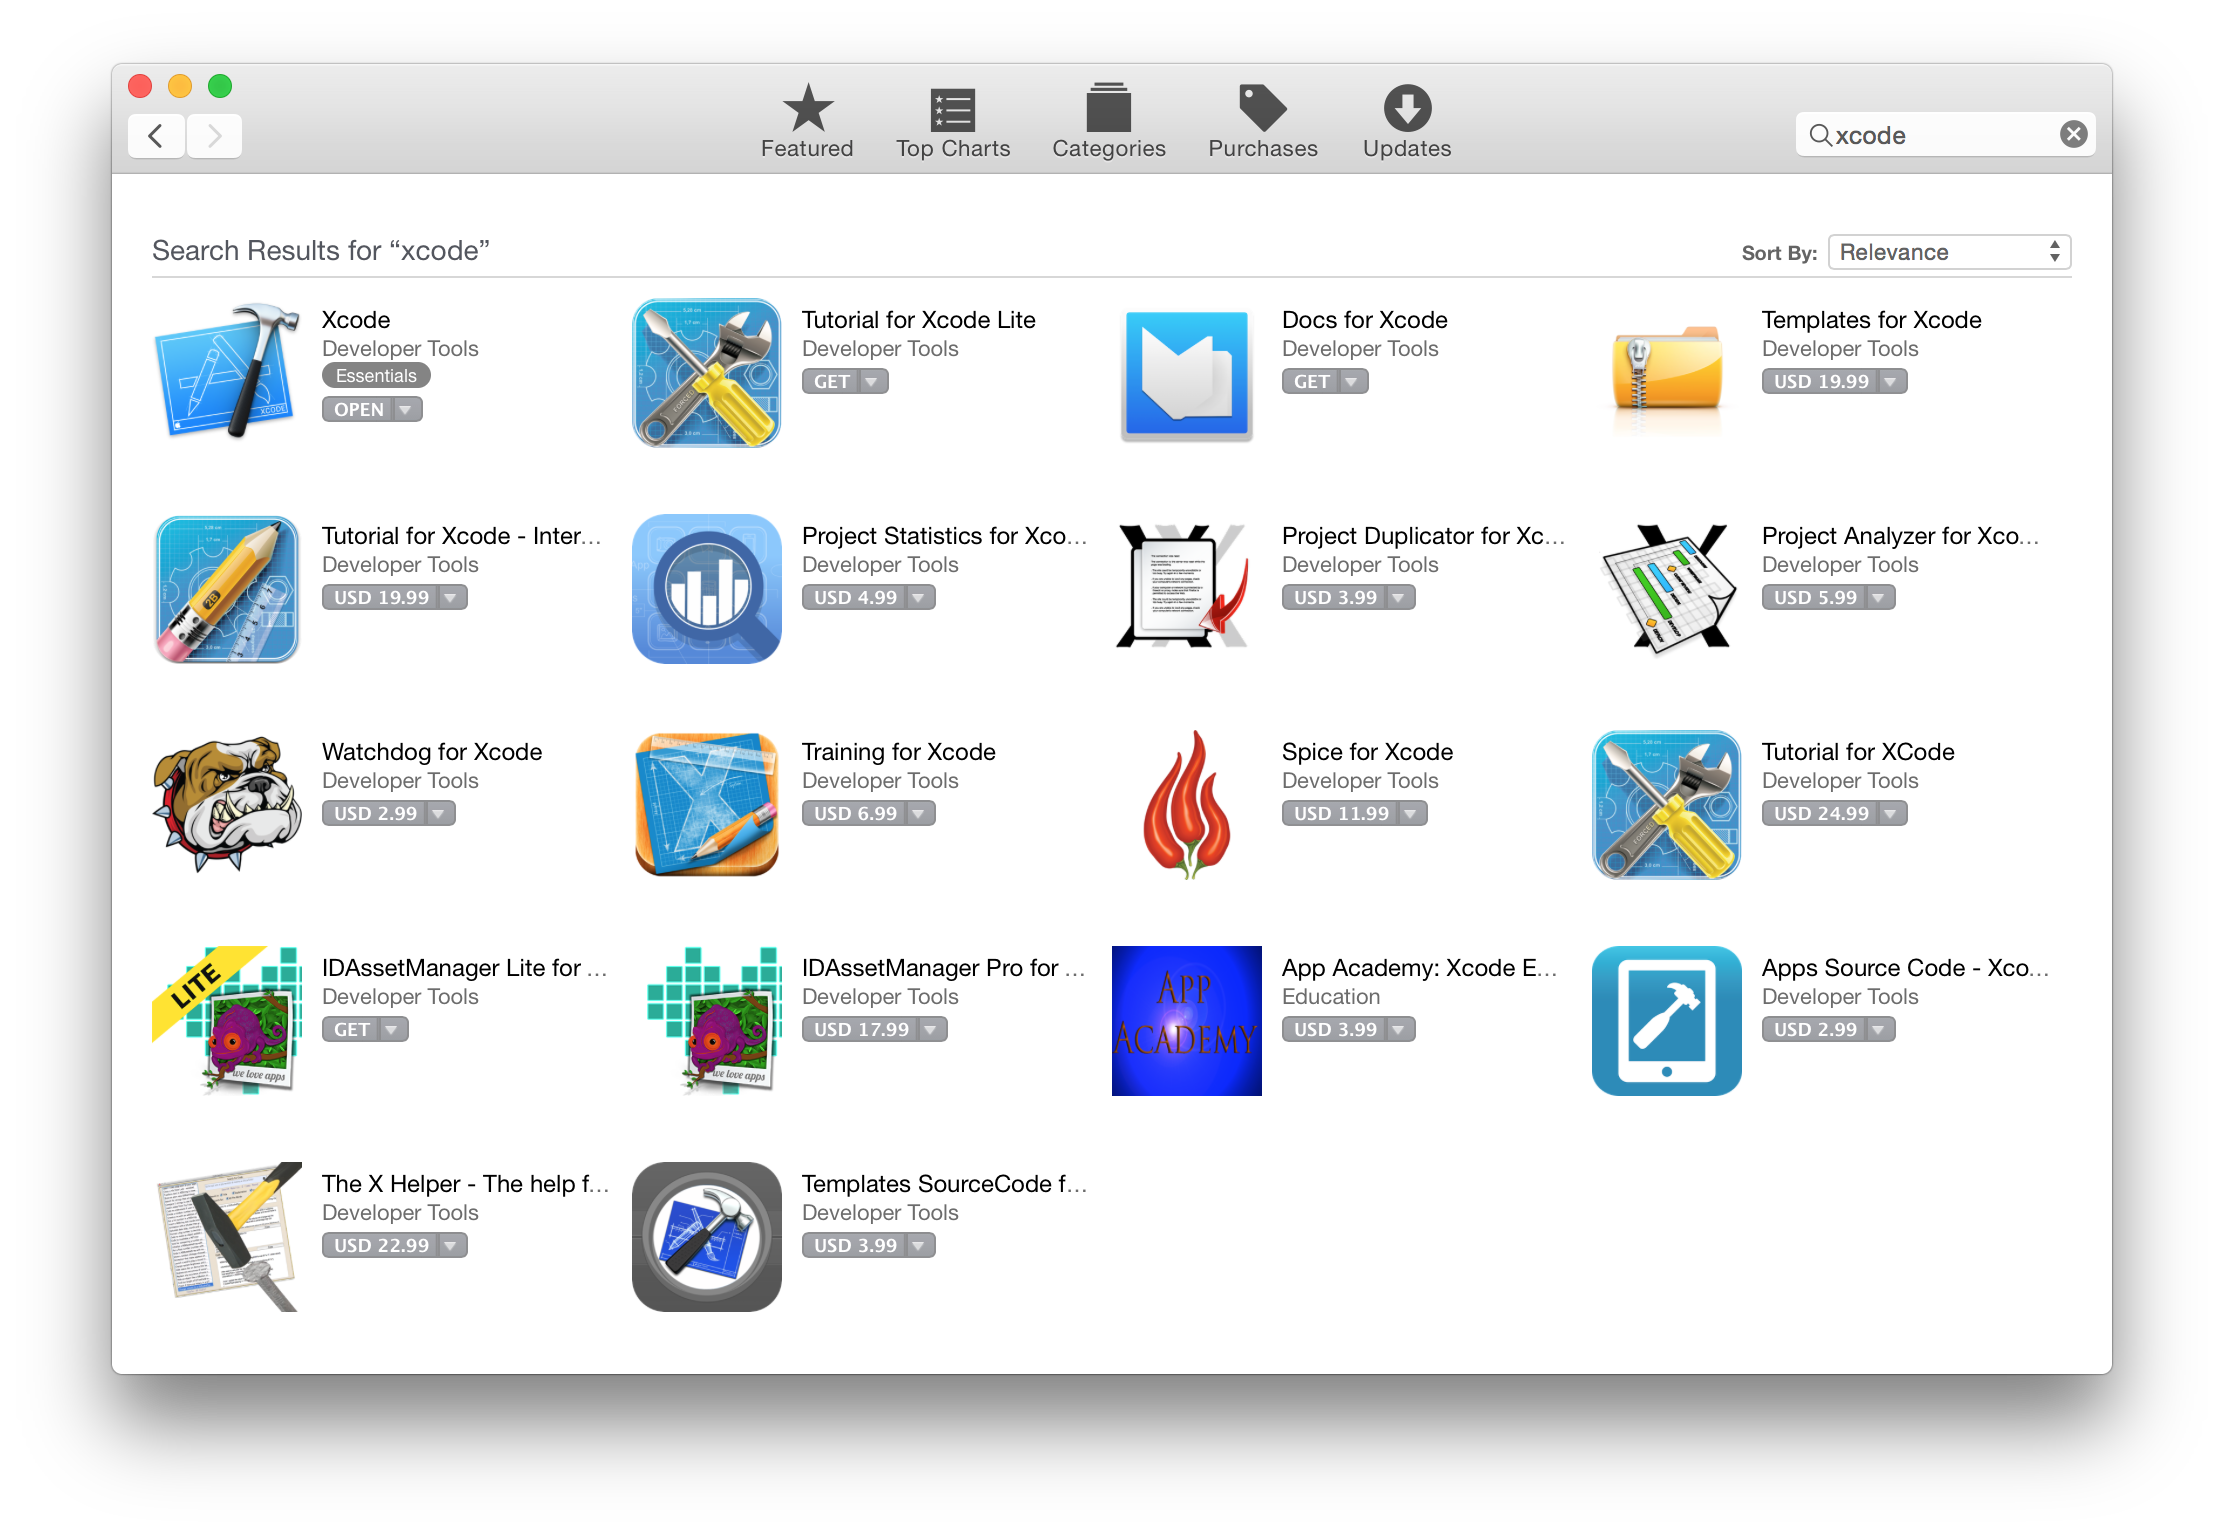
\includegraphics[width=150mm]{pic/search_xcode.png}
  \caption{Результаты поискового запроса <<Xcode>> \\ в Mac App Store}
  \label{pic:search_xcode}
\end{figure}


\subsection{Создание проекта}
После загрузки и установки Xcode создадим проект. Для этого проделаем
следующие действия:
\begin{itemize}
  \item выбрать File $\rightarrow$ New $\rightarrow$ Project...;
  \item выбрать OS X $\rightarrow$ Cocoa Application, нажать кнопку Next;
  \item далее нужно заполнить поля так, как это показано
    на рисунке~\ref{pic:create_project} и нажать кнопку Next.
\end{itemize}

\begin{figure}[h!]
  \centering
  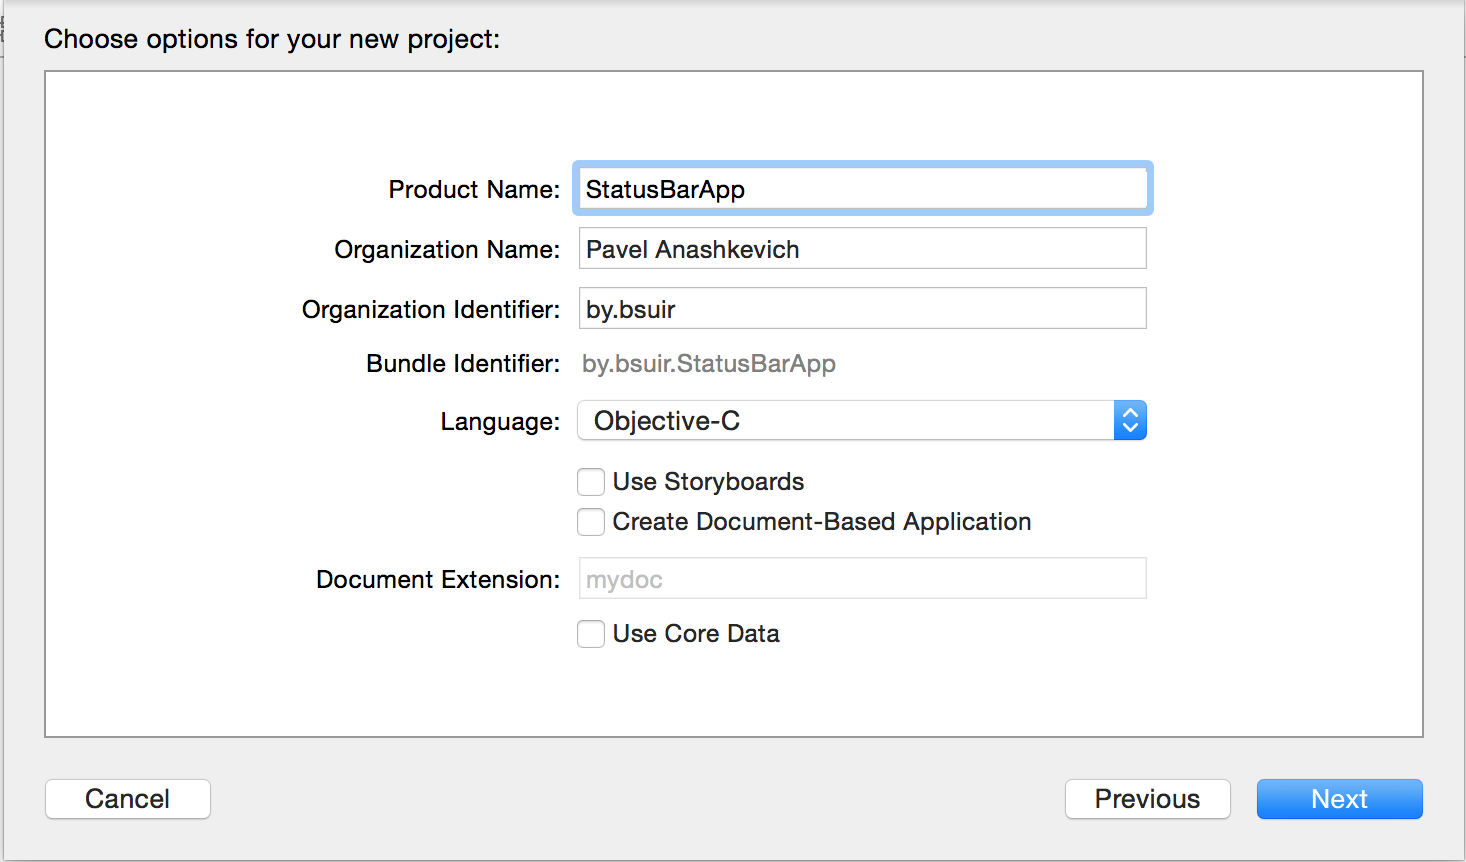
\includegraphics[width=150mm]{pic/create_project.png}
  \caption{Создание нового проекта в Xcode}
  \label{pic:create_project}
\end{figure}

После того, как пользователь выберет место для сохранения проекта, Xcode
сгенерирует новый проект. Рассмотрим структуру директорий этого проекта.
В корневой директории созданного проекта находится три папки: StatusBarApp,
StatusBarAppTests, Products. StatusBarApp содержит в себе файлы AppDelegate.m,
AppDelegate.h, MainMenu.xib и папки Images.xcassets и Supporting Files. Папка
Supporting Files содержит файлы main.m и Info.plist.

Файл Info.plist --- структурированный текстовый файл, который содержит основную
информацию о конфигурации приложения. Сам файл, как правило, кодируется с
использованием кодировки Unicode UTF-8 и содержит структурированную информацию
в формате XML~\cite{appledoc_plist}.

Функция \texttt{main()}, находящаяся в файле main.m является точкой входа в код программы.
Содержимое файла main.m представлено на рисунке~\ref{lst:main}
\begin{lstlisting}[basicstyle=\scriptsize\ttfamily,
                   numberstyle=\scriptsize\ttfamily,
                   xleftmargin=7mm,
                   language=C++,caption=Содержимое файла main.m,
                   label=lst:main]
#import <Cocoa/Cocoa.h>

int main(int argc, const char * argv[]) {
    return NSApplicationMain(argc, argv);
}
\end{lstlisting}

Функция \texttt{NSApplicationMain()} создаёт объекты, необходимые для работы приложения.
Сначала она создаёт единственный экземпляр класса \texttt{NSApplication}, затем создаёт
экземпляр класса \texttt{NSAppDelegate} и назначает его делегатом приложения.
Стоит отметить, что этот файл, как правило, является неизменным для всех
разрабатываемых приложений на языке Objective-C.

Папка Images.xcassets используется для хранения изображений, используемых
в приложении. Директория StatusBarAppTests используется для написания тестов
для приложения, папка Products сохраняет результаты проделанной работы в виде
файла StatusBarApp.app, который в дальнейшем может использоваться для
размещения приложения в Mac App Store.


\subsection{Разработка дизайна приложения}

Приступим к разработке дизайна приложения, а именно, к разработке дизайна журнала
с записями о нажатых клавишах. Для этого откроем файл MainMenu.xib
в Interface Builder. Выберем элемент класса \texttt{NSWindow} для редактирования,
нанесём на него две кнопки Push Button и текстовый контейнер TextView.

Изменим подписи у элементов Push Button. Для этого сделаем кнопку
активной, в правой части окна Xcode выберем Attributes Inspector и изменим
поле Title. Тоже самое проделаем для второй кнопки. Для окна зададим название
<<Обработка событий клавиатуры>>, изменим пропорции, а также пропорции
элемента TextView и расположение кнопок.

Далее необходимо связать визуальные элементы, отображаемые в файле MainWindow.xib
с объектами в коде приложения. Для этого в полной мере воспользуемся возможностями
Xcode: откроем двухоконный режим, в левой части которого будет располагаться
открытый в Interace Builder файл MainWindow.xib, а в правой файл AppDelegate.m.
При помощи мыши <<перетащим>> элементы Push Button и TextView в файл делегата
приложения (должна быть нажата клавиша \texttt{Ctrl}). Для элементов типа Push Button
создадим IBAction, а для TextView --- IBAction и IBOutlet.

IBOutlet служит для связывания ссылки на объект, определённой в коде на Objective-C,
с экземпляром объекта в Interface Builder.

IBAction служит для связывания события, посылаемого объекту, с определённым
в коде методом.

Фрагмент кода, иллюстрирующий связывание TextView с помощью IBOutlet приведен
на рисунке~\ref{lst:iboutlet}.
\begin{lstlisting}[basicstyle=\scriptsize\ttfamily,
                   numberstyle=\scriptsize\ttfamily,
                   xleftmargin=7mm,
                   language=C++,caption=Связывание TextView с помощью IBOutlet,
                   label=lst:iboutlet]
@property (unsafe_unretained) IBOutlet NSTextView *logTextView;
\end{lstlisting}

Интерфейс журнала с записями о нажатых клавишах в системе представлен
на рисунке~\ref{pic:log_window}.
\begin{figure}[h!]
  \centering
  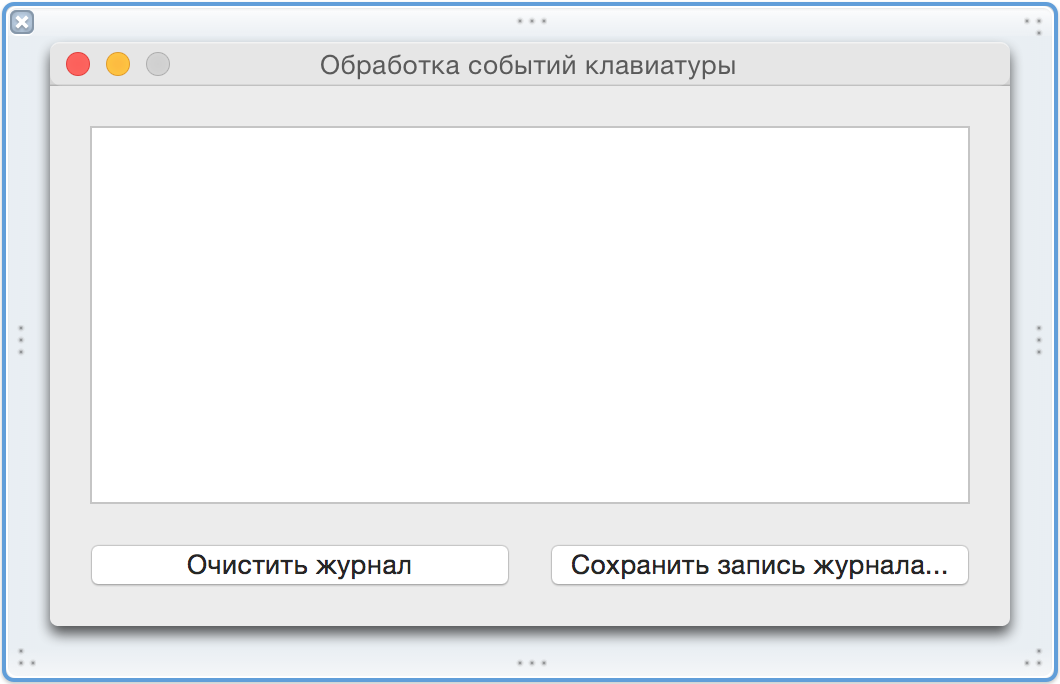
\includegraphics[width=150mm]{pic/log_window.png}
  \caption{Интерфейс журнала с записями о \\ нажатых клавиш в системе}
  \label{pic:log_window}
\end{figure}

\subsection{Разработка программной части приложения}

В коде на Objective-C создадим меню, которое будет отображаться при нажатии на
иконку приложения в статус баре рабочего стола OX X. Вынесем команды, описывающие
меню в функцию, назовём её constructMenu. Фрагмент функции \texttt{constructMenu:}
представлен на рисунке~\ref{lst:construct_menu}.
\begin{lstlisting}[basicstyle=\scriptsize\ttfamily,
                   numberstyle=\scriptsize\ttfamily,
                   xleftmargin=7mm,
                   language=C++,caption=Фрагмент функции \texttt{constructMenu:},
                   label=lst:construct_menu]
- (void)constructMenu {
    menu = [[NSMenu alloc] init];

    statusBarItem = [[NSStatusBar systemStatusBar] statusItemWithLength:NSVariableStatusItemLength];
    [statusBarItem setImage:[NSImage imageNamed:@"app_image"]];
    [statusBarItem setMenu:menu];
    [statusBarItem setHighlightMode:NO];

    menuItem = [[NSMenuItem alloc] init];
    [menuItem setTitle:@""];
    [menuItem setKeyEquivalent:@"R"];
    [menuItem setState:NSOnState];
    [menuItem setAction:@selector(changeStatus:)];
    [menu addItem:menuItem];
    [menu addItem:[NSMenuItem separatorItem]];
    ...
}
\end{lstlisting}

Обработку нажатий клавиатуры реализуем внутри блока, являющегося одним из
параметров функции \texttt{addGlobalMonitorForEventsMatchingMask:}. Фрагмент кода,
реализующий обработку нажатия клавиш на клавиатуре приведен на рисунке~\ref{lst:keyPressed}.
\begin{lstlisting}[basicstyle=\scriptsize\ttfamily,
                   numberstyle=\scriptsize\ttfamily,
                   xleftmargin=7mm,
                   language=C++,caption={Фрагмент кода, реализующий обработку \\
                      нажатия клавиш на клавиатуре},
                   label=lst:keyPressed]
[NSEvent addGlobalMonitorForEventsMatchingMask:NSKeyDownMask handler:^(NSEvent *event) {
    [self keyPressed:event];
}];

- (void)keyPressed:(NSEvent *)event {
    ...
}
\end{lstlisting}

Для очисти журнала воспользуемся методом \texttt{replaceCharactersInRange:} экземпляра
класса \texttt{NSTextView}. Фрагмент кода, реализующий очистку журнала представлен
на рисунке~\ref{lst:clearLog}.
\begin{lstlisting}[basicstyle=\scriptsize\ttfamily,
                   numberstyle=\scriptsize\ttfamily,
                   xleftmargin=7mm,
                   language=C++,caption={Фрагмент кода, реализующий очистку журнала},
                   label=lst:clearLog]
- (IBAction)clearLogButton:(id)sender {

    NSRange textRange = NSMakeRange(0, [[self.logTextView string] length]);
    [self.logTextView replaceCharactersInRange:textRange withString:@""];
}
\end{lstlisting}

Для сохранения журнала в файл воспользуемся конструкцией блоков, пример приведен
на рисунке~\ref{lst:saveLog}.
\begin{lstlisting}[basicstyle=\scriptsize\ttfamily,
                   numberstyle=\scriptsize\ttfamily,
                   xleftmargin=7mm,
                   language=C++,caption={Использование блока для сохранения файла журнала},
                   label=lst:saveLog]
- (IBAction)saveLogButton:(id)sender {
    NSSavePanel *savePanel = [NSSavePanel savePanel];
    NSString *fileName = [NSString stringWithFormat:@"log_%i.log", logNumber];

    [savePanel beginSheetModalForWindow:self.logWindow completionHandler:^(NSInteger result) {
        if (result == NSFileHandlingPanelOKButton) {

            ...
        }
    }];
}
\end{lstlisting}

Исходный текст разработанной программы расположен в приложении~А.

\pagebreak
